\documentclass[UTF8]{ctexart}
\usepackage{xcolor}
\usepackage{graphicx}
\usepackage{geometry}
\usepackage{section}
\usepackage{subfigure}
\usepackage{float}
\usepackage{listings}
\geometry{top=3.0cm, bottom=1.0cm, right=1.5cm, left=1.5cm}

%\lstset{basicstyle=\sffamily, keywordstyle=\bfseries,commentstyle=\rmfamily\itshape,stringstyle=\ttfamily }
\lstset{numbers=left,
	numberstyle=\tiny,
	basicstyle=\sffamily, 
	keywordstyle=\bfseries,
	commentstyle=\rmfamily\itshape,
	stringstyle=\ttfamily
	keywordstyle=\color{blue!70}, commentstyle=\color{red!50!green!50!blue!50},
	frame=shadowbox,
	rulesepcolor=\color{red!20!green!20!blue!20}
}



\title{\huge{实验三:滤波器设计和滤波器的特性分析}}
\author{\textbf{PB18020520 \qquad 刘洪健}}
\date{\today}

\begin{document}
\maketitle
\tableofcontents
\section{实验目的}
\begin{enumerate}
	\item 掌握matlab中滤波器设计工具fdatool的方法
	\item 掌握IIR滤波器设计的方法
	\item 掌握FIR滤波器设计的方法
	\item 了解IIR 和 FIR 滤波器的特性
	\item 掌握滤波器性能分析的方法
	\item 掌握sptool工具的使用
\end{enumerate}
\section{实验内容}
\subsection{IIR滤波器}
\subsubsection{高通滤波器}
\hspace*{2em}利用Chebyshev模型设计,按照要求:$f_p=0.3Hz \quad {\alpha}_p=0.8dB \quad f_s=0.2Hz \quad {\alpha}_s=20dB$

利用matlab的cheby函数等设计,\textbf{代码如下}
\begin{lstlisting}[language=matlab]
	Fs = 1;  % Sampling Frequency

	fs = 0.2*2;         % Stopband 
	fp = 0.3*2;         % Passband 
	As = 20;          % Stopband Attenuation (dB)
	Ap = 0.8;         % Passband Ripple (dB)
	[n, Wn] = cheb1ord(fp, fs, Ap, As);
	[b, a] = cheby1(n, Ap, Wn, 'high');
	fvtool(b,a);
\end{lstlisting}
得到的H(Z)系数为

b:  0.0262   -0.1047    0.1570   -0.1047    0.0262 \\
\hspace*{2em}a:  1.0000    1.5289    1.6537    0.9452    0.2796\\
\[
H(Z)=\frac{0.0262-0.1047Z^{-1}+0.157Z^{-2}-0.1047Z^{-3}+0.0262Z^{-4}}{1+1.5289Z^{-1}+1.6537Z^{-2}+0.9452Z^{-3}+0.2796Z^{-4}}
\]
利用fvtool工具查看其幅频特性曲线,如下图
\begin{figure}[H]
	\centering
	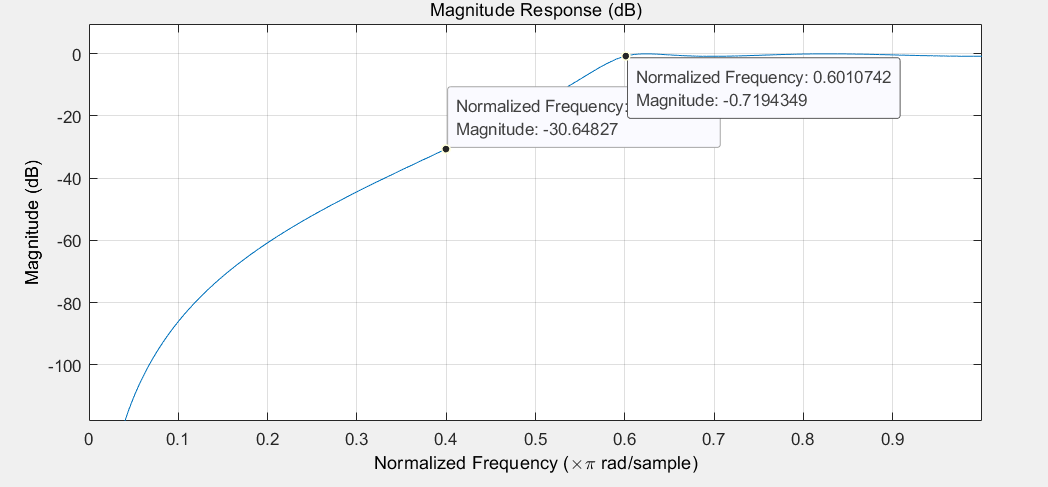
\includegraphics[scale=0.8]{figs/iir1}
	\caption{IIR高通滤波器}
\end{figure}
可以看出,在通带和阻带的起伏均满足要求。同时,根据幅频特性曲线,在通带内并不是严格下降的,而是有一定波纹的,也符合chebyshev模型的特点,同时滤波器只用了5阶就实现了要求。
\subsubsection{低通滤波器}
设计数字低通滤波器,其中的性能要求是::$f_p=0.2Hz \quad {\alpha}_p=1dB \quad f_s=0.3Hz \quad {\alpha}_s=25dB$\\
我采用Butterworth法设计,\textbf{代码如下}
\begin{lstlisting}[language=matlab]
	Fs = 1;  % Sampling Frequency
	
	fs = 0.3*2;         % Stopband 
	fp = 0.2*2;         % Passband 
	As = 25;          % Stopband Attenuation (dB)
	Ap = 1;         % Passband Ripple (dB)
	[n, Wn] = buttord(fp, fs, Ap, As);
	[b, a] = butter(n, Wn);
	fvtool(b,a);
\end{lstlisting}
得到的H(Z)系数为\\
\hspace*{2em}b:  0.0179    0.1072    0.2681    0.3575    0.2681    0.1072    0.0179 \\
\hspace*{2em}a:  1.0000   -0.6019    0.9130   -0.2989    0.1501   -0.0208    0.0025 \\
\[
H(Z)=\frac{0.0179+0.1072Z^{-1}+0.2681Z^{-2}+0.3575Z^{-3}+0.2681Z^{-4}+0.1072Z^{-5}+0.0179Z^{-6}}{1-0.6019Z^{-1}+0.913Z^{-2}-0.2989Z^{-3}+0.1501Z^{-4}-0.0208Z^{-5}+0.0025Z^{-6}}
\]
利用fvtool查看其幅频特性曲线,如下图
\begin{figure}[H]
	\centering
	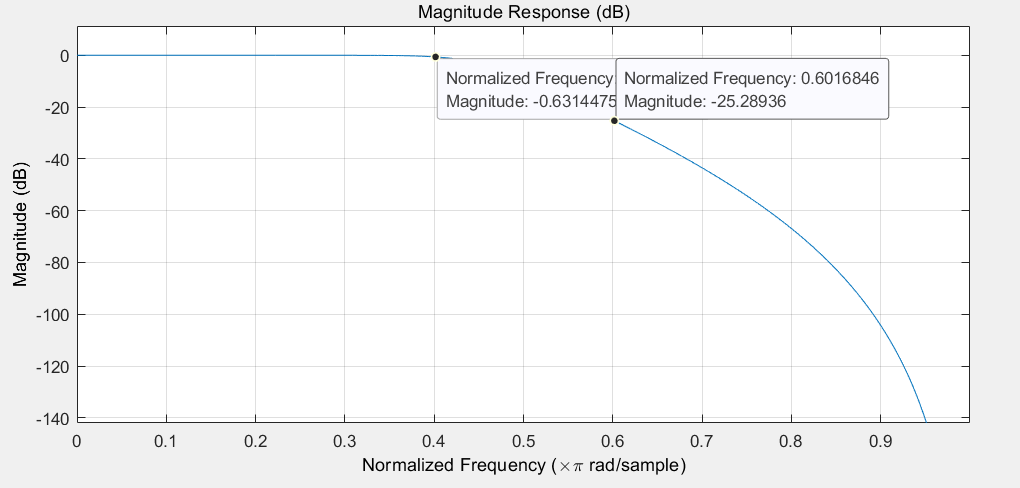
\includegraphics[scale=0.8]{figs/iir2}
	\caption{IIR低通滤波器}
\end{figure}
可以看出,在通带和阻带的起伏均满足要求。同时,根据幅频特性曲线,幅频曲线严格下降,符合Butterworth模型。
\subsubsection{Butterworth带通滤波器}
利用matlab设计带通滤波器,其中的性能要求是:$f_{p1}=20kHz \quad f_{p2}=30kHz \quad f_{s1}=15kHz \quad {\alpha}_p=1dB \quad {\alpha}_s=40dB \quad T_s=10us \quad f_s=\frac{1}{T_s}=100kHz$

同样使用matlab的Buttored函数设计Butterworth模型的滤波器,代码如下
\begin{lstlisting}[language=matlab]
	Fs=1e5;
	fp1=20e3*2;
	fp2=30e3*2;
	fs1=15e3*2;
	fs2=35e3*2;
	Ap=1;
	As = 40;
	
	[n, Wn] = buttord([fp1 fp2]/Fs, [fs1 fs2]/Fs, 1, 40);
	[b,a] = butter(n, Wn);
	fvtool(b,a);
\end{lstlisting}
 得到的H(Z)的系数为\\
 \hspace*{2em}b: 0.0002 0   -0.0014  0 0.0042  0 -0.0071 0 0.0071  0   -0.0042  0    0.0014    0   -0.0002\\
 \hspace*{2em}a: 1.0000 -0.0000  3.7738 -0.0000  6.5614   -0.0000    6.6518   -0.0000    4.2030   -0.0000    1.6437   -0.0000    0.3666   -0.0000   0.0359\\
 \[
 H(Z)=\frac{0.0002-0.0014Z^{-2}+0.0042Z^{-4}-0.0071Z^{-6}+0.0071Z^{-8}-0.0042Z^{-10}+0.0014Z^{-12}-0.0002Z^{-14}}{1+3.7738Z^{-2}+6.5614Z^{-4}+6.6518Z^{-6}+4.2030Z^{-8}+1.6437Z^{-10}+0.3666Z^{-12}-0.0359Z^{-14}}
 \]
 利用fvtool查看其幅频特性曲线,如下图
 \begin{figure}[H]
 	\centering
 	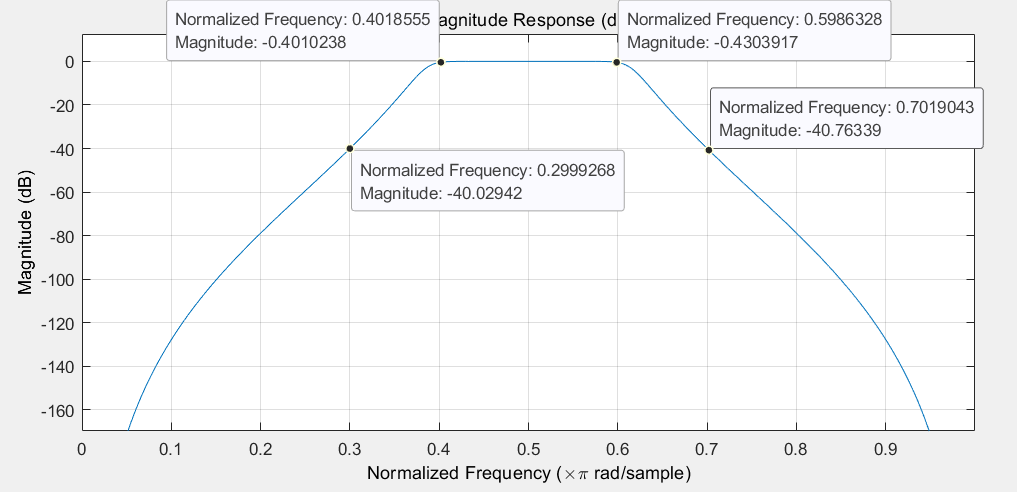
\includegraphics[scale=0.8]{figs/iir3}
 	\caption{Butterworth带通滤波器}
 \end{figure}
可以出,在通带的起伏和阻带的衰减都满足性能要求。正如Butterworh模型的理论一样,在通带十分平坦,且从通带到阻带是单调下降的。
\subsection{FIR滤波器}
\subsubsection{带通滤波器}
利用hanning窗设计线性相位带通滤波器,其性能要求为$w_1=0.3\pi \qquad w_2=0.5\pi \qquad {\alpha}_p=3dB  \qquad {\alpha}_s=20dB  $\\
观察N=15和45时的性能差异
下面是的设计的代码
\begin{lstlisting}][language=matlab]
	N=15;% 45
	w1=0.3;
	w2=0.5;
	Window=hanning(N + 1);
	b=fir1(N, [w1 w2],Window);
	figure(1);
	freqz(b,1);
\end{lstlisting}
查看两者的幅频和相频响应曲线
\begin{figure}[H]
	\centering
	\subfigure[N=15]{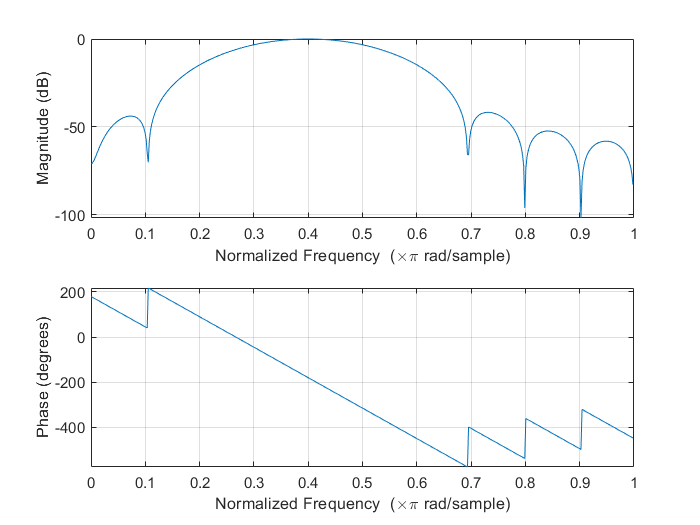
\includegraphics[scale=0.43]{figs/fir15}}\quad
	\subfigure[N=45]{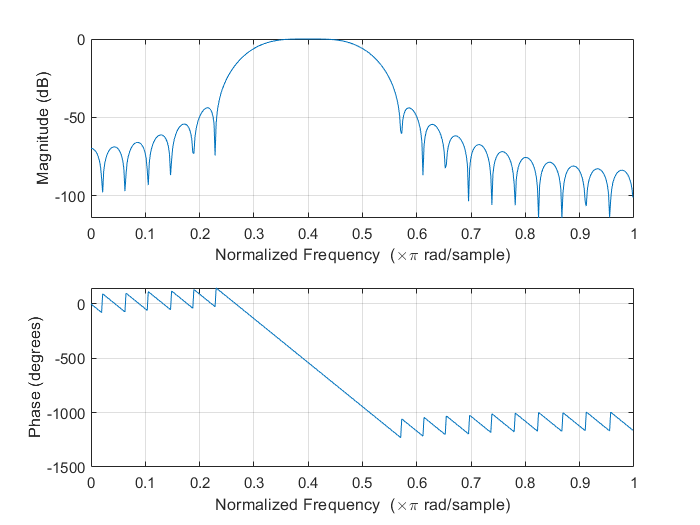
\includegraphics[scale=0.43]{figs/fir45}}
	\caption{Hannig窗}
\end{figure}
从图中可以看出,利用FIR确实可以较好地设计线性相位滤波器.对于同一个滤波器,当N越大时,其过渡带越短,幅频响应下降地越快。对于Hanning窗,其过渡带大小等于主瓣宽度$\frac{8\pi}{N}$,和阶数N成反比。\\
将窗函数换做矩形窗和Blackman窗,再查看系统函数的幅频响应和相频响应,如下图
\begin{figure}[H]
	\centering
	\subfigure[矩形窗N=15]{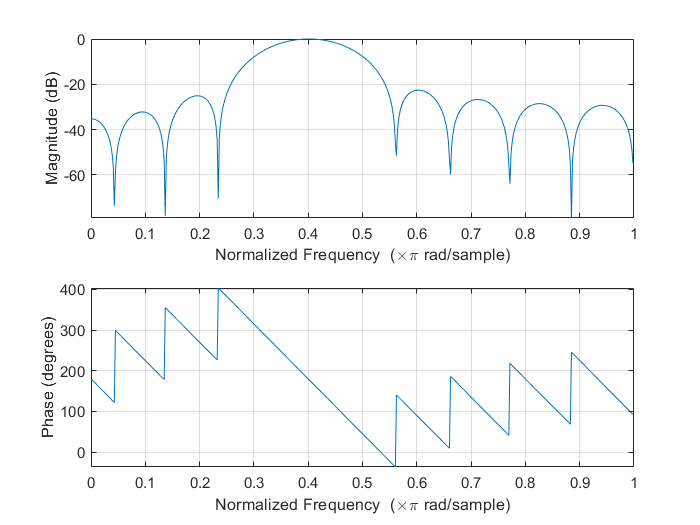
\includegraphics[scale=0.43]{figs/box15}}\quad
	\subfigure[矩形窗N=45]{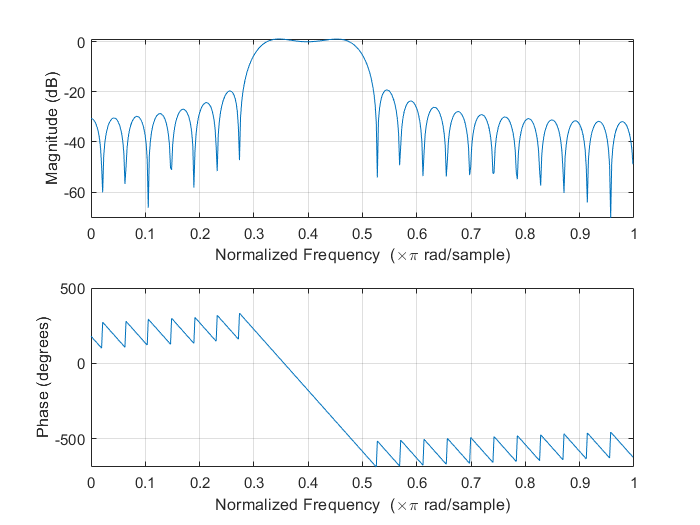
\includegraphics[scale=0.43]{figs/box45}}
	\subfigure[Blackman窗N=15]{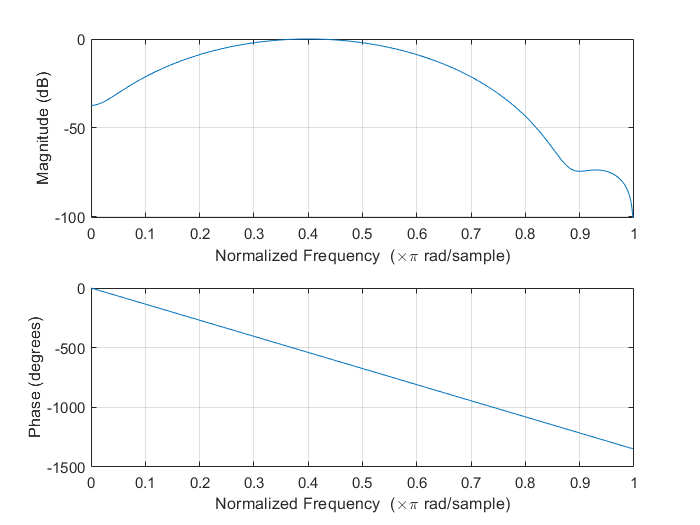
\includegraphics[scale=0.43]{figs/black15}}\quad
	\subfigure[Blackman窗N=45]{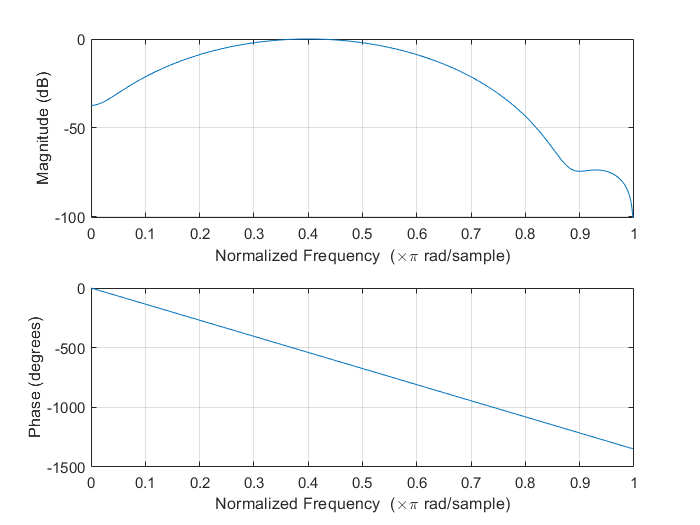
\includegraphics[scale=0.43]{figs/black45}}	
	\caption{矩形窗和Blackman窗的带通滤波器}
\end{figure}
综合来看,
\begin{itemize}
	\item 上面的FIR滤波器都反应出良好的线性相位特性
	\item  在过渡带宽度上,Hanning窗为$\frac{8\pi}{N}$,矩形窗为$\frac{4\pi}{N}$,Blackman窗为$\frac{12\pi}{N}$,相同阶数下,矩形窗过渡带最短,下降更快。而所以窗函数滤波器的过渡带都随着阶数N的增加而下降。
	\item 从波纹来看,Blackman窗在阻带较为光滑,波纹较少,而另外两种窗都有较多的波纹。在阻带上,blackman窗阻带衰减最多。
\end{itemize}
\subsubsection{Kaiser窗设计特定滤波器}
更具所需的频率响应图形,设计Kaiser窗的FIR滤波器,并且观察$\beta$参数的影响
其中的幅频响应和相频响应如下
\begin{figure}[H]
	\centering
	\subfigure[$\beta$=4]{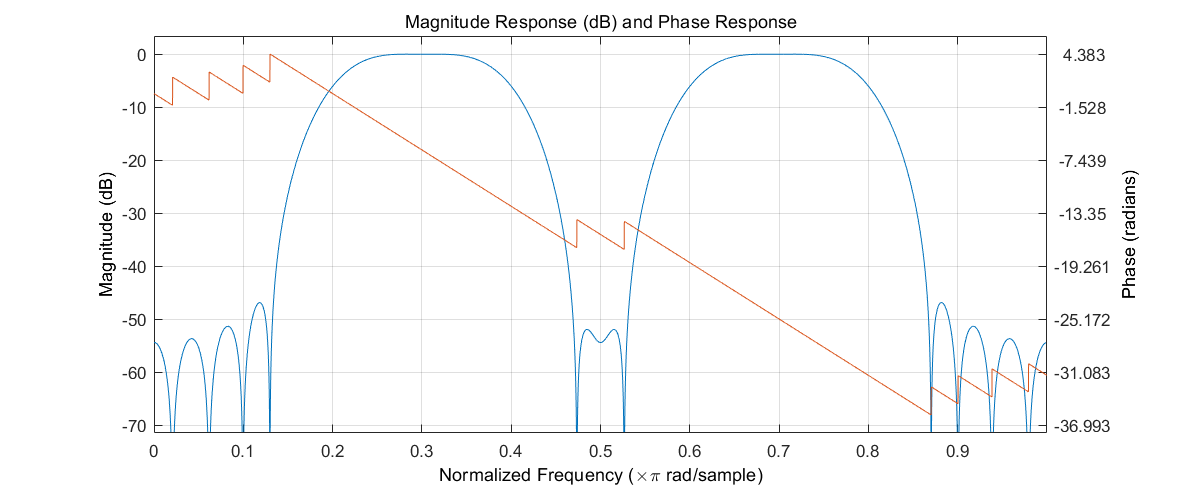
\includegraphics[scale=0.28]{figs/kaiser}}\quad
	\subfigure[$\beta$=8]{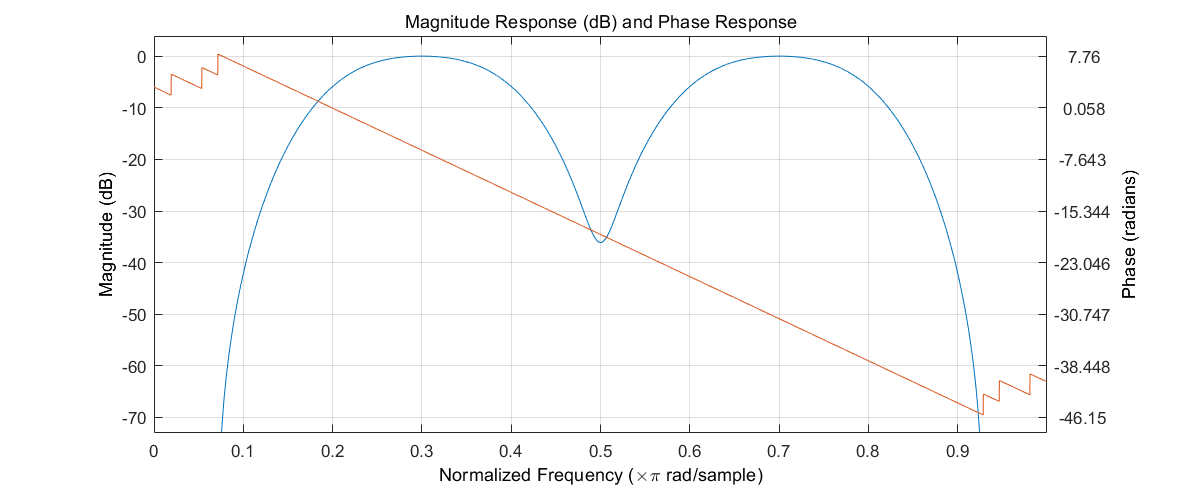
\includegraphics[scale=0.28]{figs/kaiser8}}
	\caption{Kaiser窗设计特定的滤波器}
\end{figure}
通过观察,$\beta$越大,旁瓣电平越低,过渡带后幅频响应衰减越快,但是主瓣宽度会变大。
\subsection{滤波器性能的比较}
FIR和IIR滤波器设计3.3.1中不同要求的性能比较,我主要采用了fvtool工具来查看滤波器的幅频响应,相频响应,群延时,零极点分布图,相位延时等。\\
\textbf{根据性能指标设计FIR的过程}:

\begin{enumerate}
	\item 首先根据阻带的衰减要求选择特定的窗函数
	\item 根据过渡带的宽度确定滤波器的阶数$N=\frac{k\pi}{\delta w}$
	\item 在FIR滤波器中存在肩峰和过冲,所以在matlab中输入截止频率时要有一定的裕量在设计截止频率时还要考虑肩峰的影响,$w_c'=w_c-\frac{2\pi}{N}$
\end{enumerate}
\textbf{1.幅频响应,相频响应,群延时(以高通滤波器为例)}
\begin{figure}[H]
	\centering
	\subfigure[IIR,N=5]{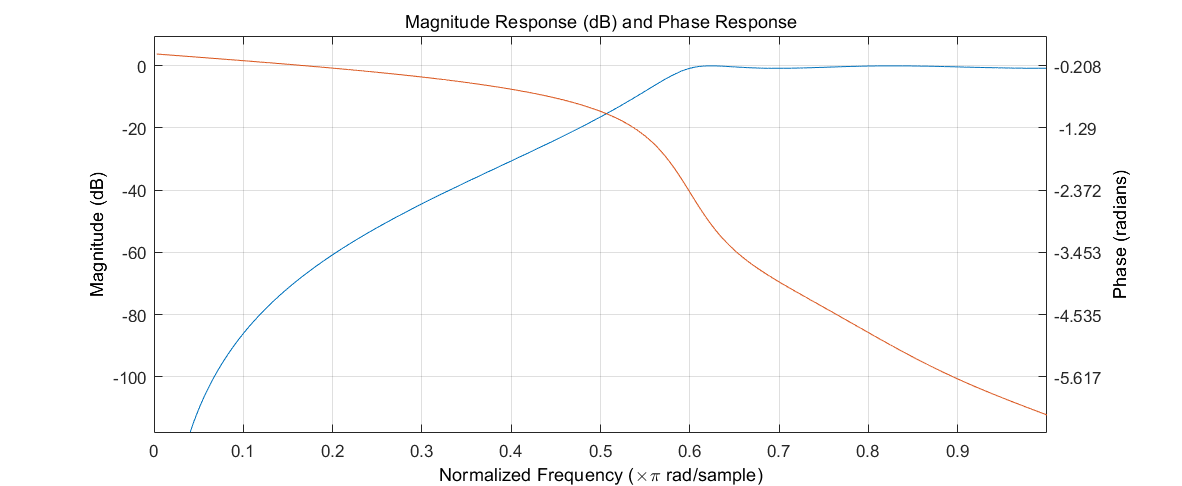
\includegraphics[scale=0.25]{figs/gaoiir}}\quad
	\subfigure[FIR, N=40]{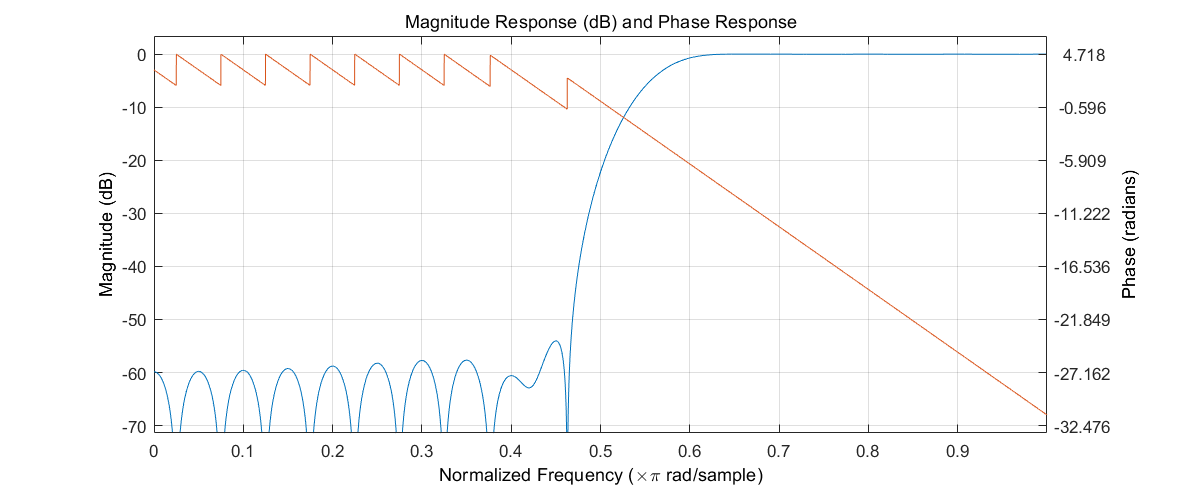
\includegraphics[scale=0.25]{figs/gaofir}}
	\subfigure[IIR,群延时]{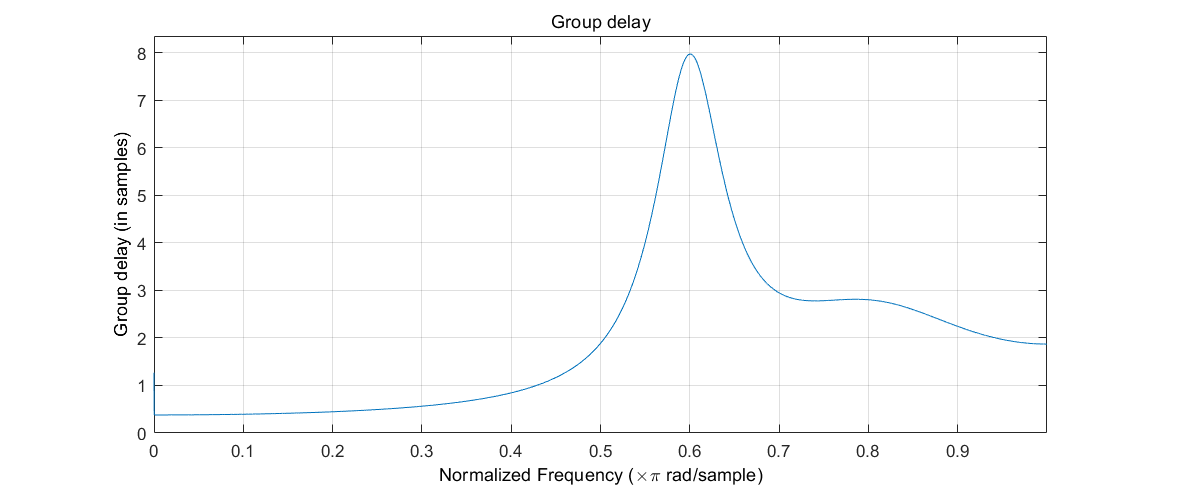
\includegraphics[scale=0.25]{figs/gaoiirgroup}}\quad
	\subfigure[FIR, 群延时]{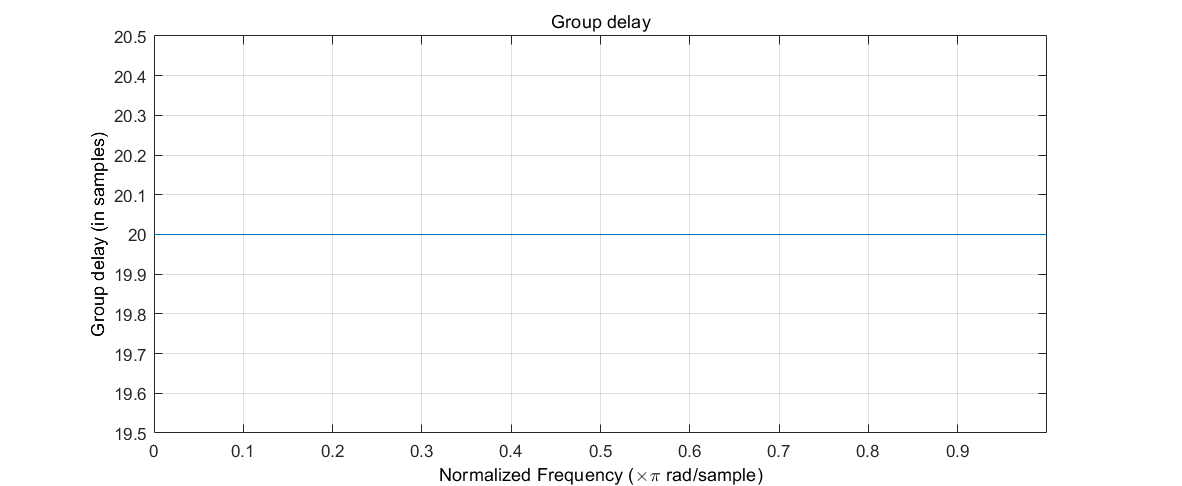
\includegraphics[scale=0.25]{figs/gaofirgroup}}	
	\caption{IIR 和 FIR的高通滤波器}
\end{figure}
\textbf{2.幅频响应,相位延迟,零极点分布(以低通滤波器为例)}
\begin{figure}[H]
	\centering
	\subfigure[IIR,N=7]{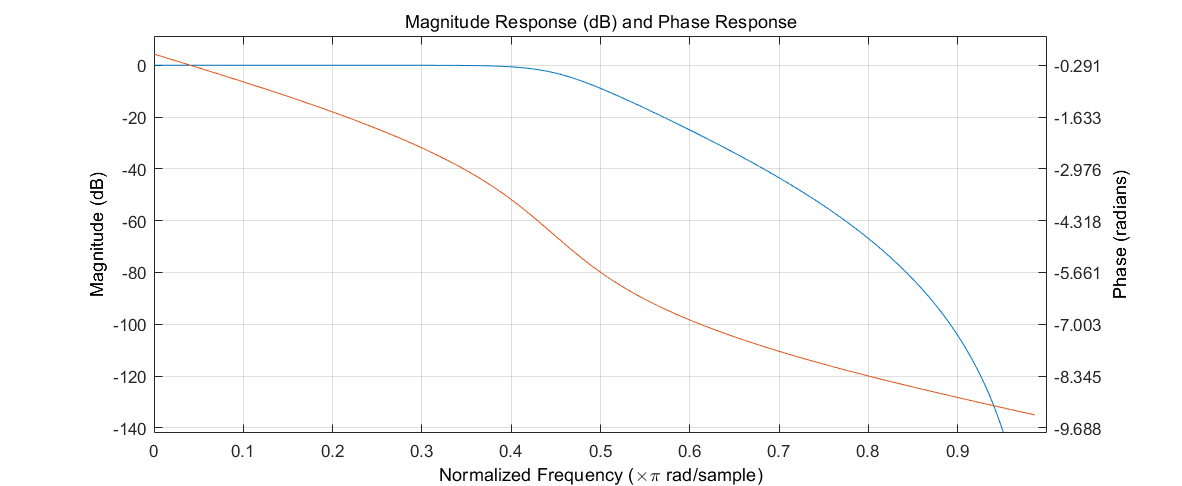
\includegraphics[scale=0.25]{figs/diiir}}\quad
	\subfigure[FIR, N=40]{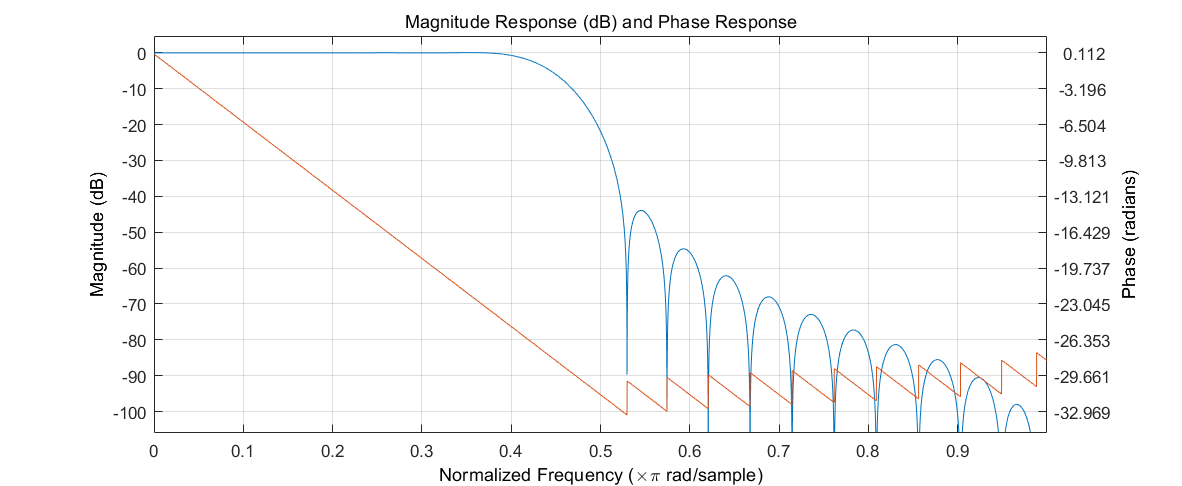
\includegraphics[scale=0.25]{figs/difir}}
	\subfigure[IIR,相位延时]{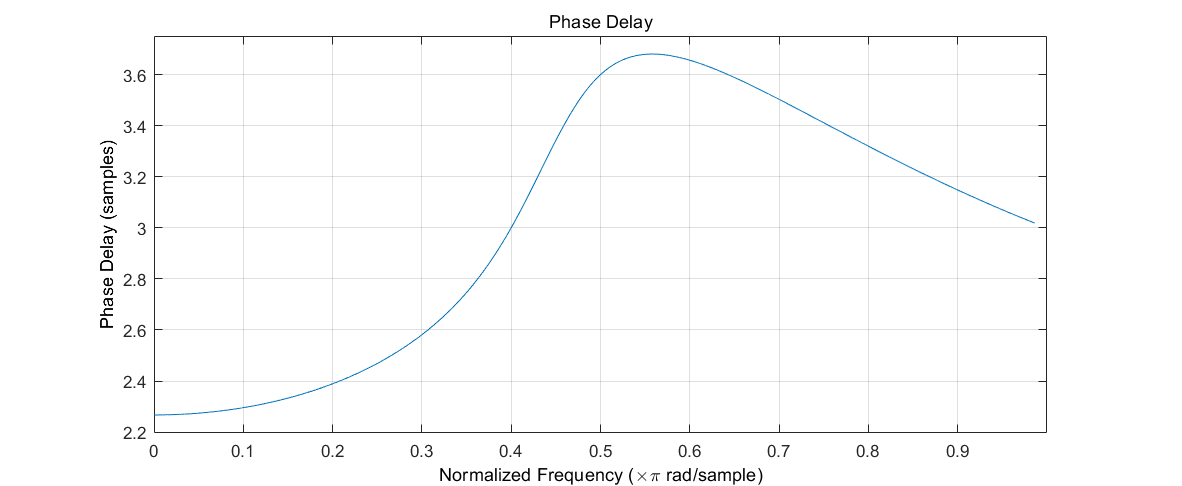
\includegraphics[scale=0.25]{figs/diiirphase}}\quad
	\subfigure[FIR, 相位延时]{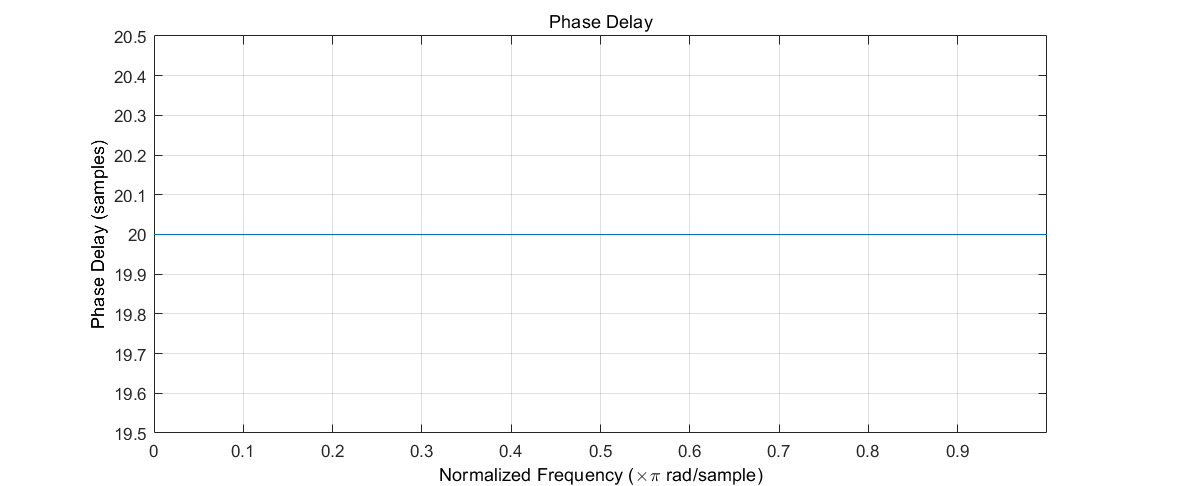
\includegraphics[scale=0.25]{figs/difirphase}}
\end{figure}
\begin{figure}[H]
	\centering	
	\subfigure[IIR,零极点]{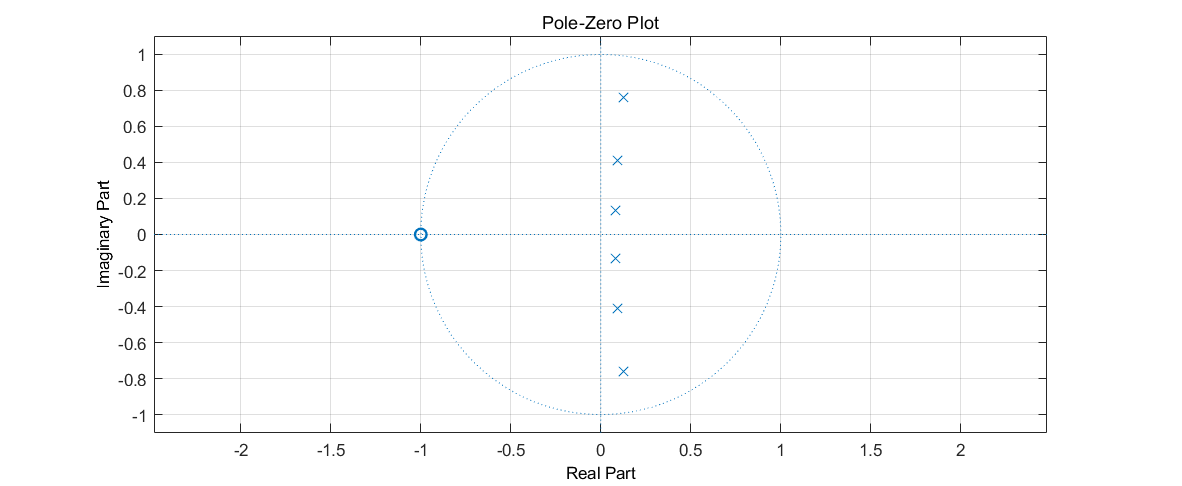
\includegraphics[scale=0.25]{figs/diiirpoint}}\quad
	\subfigure[FIR, 零极点]{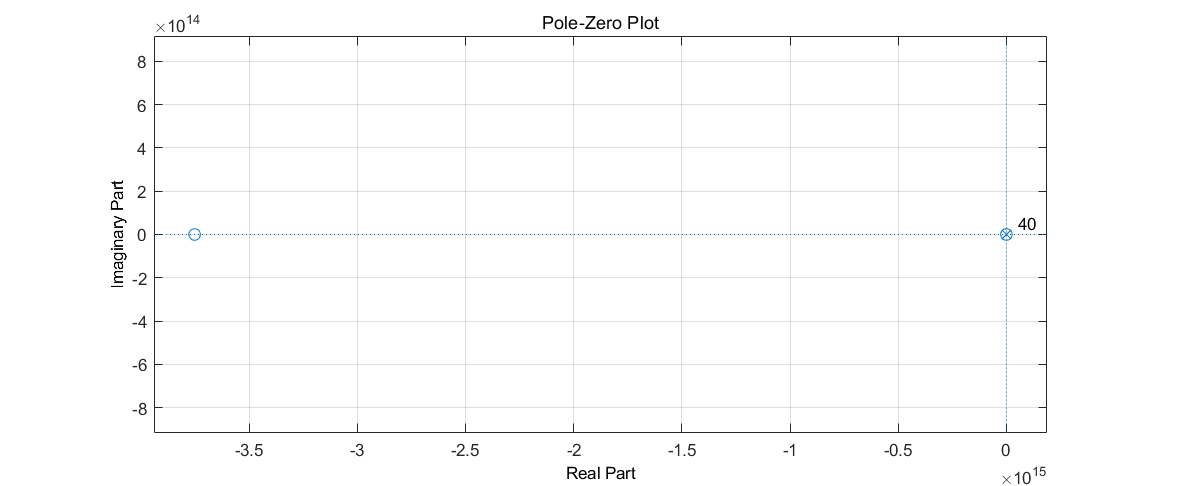
\includegraphics[scale=0.25]{figs/difirpoint}}
	\caption{IIR 和 FIR的低通滤波器}
\end{figure}
\textbf{比较分析}
\begin{itemize}
	\item 从阶数上,在满足同样的特性要求(阻带衰减,通带起伏)的情况下,FIR所需的阶数要远多于IIR。
	\item 从过渡带上看,由于FIR所需要的阶数更多,在过渡带上一般下降更快,过渡带更短,而且在过渡带阶数后会有波纹出现。因为在FIR滤波器的设计中,波纹其实是矩形脉冲和窗函数的叠加,从频域上看,矩形脉冲是无限波纹状的。而在IIR中,由于冲激序列是无限长的,所以波纹较少,单调性较好。
	\item 从相位上来看,FIR具有良好的线性相位特性,IIR则不然,这也使得在FIR的群延时为常数,IIR的群延时确实变化的。同时,可以看出FIR的相位延迟比IIR大,这也和FIR要远大于IIR阶数有关。
	\item 从零极点来看,一般单位圆上离极点近的是通带,离极点远的是通带。
	IIR滤波器的极点在单位圆内分散分布,可以通过改变极点的位置来方便地调整幅频响应。而FIR滤波器的极点集中在原点,零点在远方,想要调整幅频响应,只有提高阶数或者换一个窗函数。而零极点的分布,也决定了其相位特性,IIR是非线性相位,而FIR的极点均在原点处,其相位是线性的。
\end{itemize}
\subsection{FIR和IIR滤波器优缺点的总结}
\begin{table}[H]
	\centering
	\begin{tabular}{|c|c|c|}
		\hline
		& FIR & IIR \\ \hline
		阶数 & 较多,成本高,复杂 & 较少,成本低,复杂 \\ \hline
		阻带的波纹 & 有明显的波纹 & 不明显 \\ \hline
		零,极点分布 & 极点集中在原点,一定是稳定的,零点在远处 & 极点在单位圆内分散分布,设计时要确保稳定性 \\ \hline
		相位 & 容易实现线性相位 & 一般为非线性,但可以外加网络实现线性相位,不方便 \\ \hline
		群延时 & 较大,为常数 & 较小,变化 \\ \hline
		相位延迟 & 较大,常数 & 较小,变化 \\ \hline
		设计 & 只能通过改变阶数或者换窗函数调整幅频响应 & 容易通过改变零极点分布来调整幅频响应 \\ \hline
	\end{tabular}
\end{table}
\subsection{总结}
\hspace*{2em}本次实验,主要通过matlab实现了对IIR和FIR滤波器的设计。利用maltab的fadtool、fir1、以及Butterworh,Chebyshev等函数完成响应滤波器模型的设计,并且通过fvtool查看滤波器的特性,包括幅频特性,相频响应,群延时,相位延迟,零极点分布等。

通过实验,熟悉了在matlab平台下如何设计满足性能需求的滤波器,以及如何选用相应的模型完成滤波器设计,也进一步加深了对不同模型,例如设计IIR时的Butterworth和Chebyshev模型的特性的了解,以及在FIR中不同窗函数的区别。

同时,也对比分析了FIR和IIR的优缺点,FIR可以实现线性相位,但是所需阶数较多,幅频响应难以调整,IIR是非线性相位,容易调节零极点分布来改变幅频响应。

通过实验,提高了自己的动手能力以及对于滤波器的分析能力。在FIR中,也使用了Kisaer设计了专门的线性相位滤波器,研究了不同$\beta$参数对于滤波器的影响,拓展了知识视野。
\end{document}